

Conceptually we divide our SRL system into three stages: one stage that identifies the predicates of a sentence, one stage that identifies and classifies the arguments of these predicates, and a final stage that predicts the sense of each predicate. We should stress that this architecture is intented to illustrate a typical SRL system, and to describe the pipeline-based approach we will compare our models to. However, it does \emph{not} correspond to the way inference is performed in our proposed model---we jointly infer \emph{all} decisions described above.  

Note that while the proposed division into conceptual stages seems somewhat intuitive, it is by no means uncontroversial. In fact, for the CoNLL 2008 shared task slightly more than one half of the participants performed sense disambiguation before argument identification and classification; most other participants framed the problem in the reverse order.\footnote{However, for almost all pipeline based systems, predicate identification was the first stage of the role labelling process.} 

We define five hidden predicates for the three stages of the task. Figure \ref{fig:achitecture} illustrates these predicates and the stage they belong to. 
For predicate identification, we use the predicate \emph{isPredicate}. \emph{isPredicate(p)} indicates that the word in the position $p$ is an SRL predicate.
For argument identification and classification, we use the predicates \emph{isArgument}, \emph{hasRole} and \emph{role}. The atom \emph{isArgument(a)} signals that the word in the position $a$ is a SRL argument of some (unspecified) SRL predicate while \emph{hasRole(p,a)} indicates that the token at position $a$ is an argument of the predicate in position $p$. The predicate \emph{role(p,a,r)} corresponds to the decision that the argument in the position $a$ has the role $r$ with respect to the predicate in the position $p$. Finally, for sense disambiguation we  define the predicate \emph{sense(p,e)} which signals that predicate in position $p$ has the sense $e$. 

Before we continue to describe the formulae of our Markov Logic Network we would like to highlight the introduction of the $isArgument$ predicate mentioned above. This predicate corresponds to a decision that is usually made implicitely: a token is an argument if there exists a predicate for which plays a semantic role. Here we model this decision explicitely, assuming that there exist cases where a token clearly has to be an argument of some predicate, regardless of which predicate in the sentence this might be. It is this assumption that requires us to infer the arguments for \emph{all} predicates of a sentence at once---otherwise we cannot make sure that for a marked argument there exists at least one predicate for which it plays a semantic role.

\begin{figure}
\begin{center}
    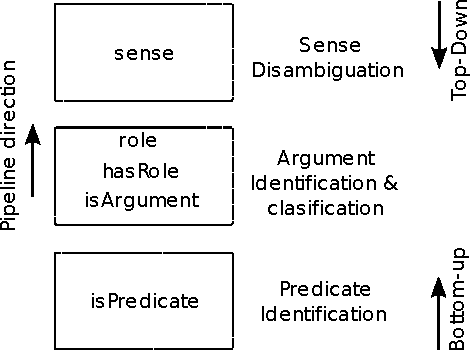
\includegraphics[scale=.70]{TaskArchitecture}
\end{center}
\caption{MLN hidden predicates divided in stages}
\label{fig:achitecture}
\end{figure}

In addition to the hidden predicates, we define observable predicates to
represent the information available in the corpus. Table \ref{tbl:o_preds}
presents these predicates. 
\begin{table}
    \small
    \centering
    \begin{tabular}{|c|p{5cm}|}
        \hline
    \emph{possiblePred(i)} & Token $i$ can be a predicate wrt. to a high recall POS tag heuristic\\\hline
    \emph{possibleArg(i)} &  Token $i$ can be an argument wrt. to a high recall POS tag heuristic\\\hline\hline
    \emph{word(i,w)}    & Token $i$ has word $w$\\\hline
    \emph{lemma(i,l)}   & Token $i$ has lemma $l$\\\hline
    \emph{ppos(i,p)}    & Token $i$ has POS tag $p$\\\hline
    \emph{cpos(i,p)}    & Token $i$ has coarse POS tag $p$\\\hline
    \emph{voice(i,v)}   & Token $i$ is verb and has voice $v$ (Active/Passive).\\\hline
    \emph{subcat(i,f)} & Token $i$ has subcategorization frame $f$\\\hline\hline
    \emph{dep(i,j,d)}     & Token $h$ is head of token $m$ and has dependency label $d$\\\hline
    \emph{palmer(i,j)}  & Token $j$ can be semantic argument for token $i$ according to high recall heuristic$^*$\\\hline
    \emph{depPath(i,j,p)}      & Dependency path between tokens $i$ and $j$ is $p$$^*$\\\hline
    \emph{depFrame(i,j,f)}     & $f$ is a syntactic (dependency) frame in which tokens $i$ and $j$ are designated as ``pivots''$^*$\\\hline
    \end{tabular}
    \caption{Observable predicates; predicates marked with $^*$ are dependency parsing-based versions for features of  }
    \label{tbl:o_preds}
\end{table}

\subsection{Local formulae}
\label{sec:local}

A formula is \emph{local} if its groundings relate any number of observed ground atoms to exactly one hidden ground atom. For example, two groundings of the local formula 
\[lemma(p,+l_1) \wedge lemma(a,+l_2) \Rightarrow hasRole(p,a)\]
can be seen in the Markov Network of Figure \ref{fig:local2}. Both connect a single  hidden \emph{hasRole} ground atom to two observed \emph{lemma} ground atoms. Note that the ``+'' prefix for variables indicates that there is a different weight for each possible pair of lemmas $(l_1,l_2)$.

The local formulae for \emph{isPredicate}, \emph{isArgument} and \emph{sense} aim to capture the relation of the tokens with their lexical and syntactic surroundings. This includes formulae such as 
\[subcat(p,+f) \Rightarrow isPredicate(p)\]
which implies that a certain token is a predicate with a weight that depends on the subcategorization frame of the token. Further local formulae are constructed using those observed predicates in table \ref{tbl:o_preds} that relate single tokens and their properties.

The local formulae for \emph{role} and \emph{hasRole} focus on properties of of the predicate and argument token---the formula illustrated in figure \ref{fig:local2} is an example of this---and on the relation between the two tokens. An example of the latter type is the formula
\[depPath(p,a,+dp) \Rightarrow role(p,a,+r)\]
which implies that token $a$ plays the semantic role $r$ with respect to token $p$, and for which the weight depends on the syntactic (dependency) path $dp$ between $p$ and $a$ and on the actual role to assign. Again, further formulae are constructed using the observed predicates in table \ref{tbl:o_preds}; however, this time we consider both predicates that relate tokens to their invidiual properties and predicates that describe the relation between tokens.

Unfortunately, the complete set of local formulae is too large to be exhaustively described in this paper. Its size results from the fact that we also consider conjunctions of several atoms as conditions, and lexical windows around tokens. Instead we refer the reader
to our MLN model files.\footnote{\url{http://anonymous.com}} They can be used both as a reference and as input to our Markov Logic
Engine,\footnote{\url{http://anonymous.com}} and thus allow the reader to easily reproduce our results. We believe that this is another advantage
of explicitly separating model and algorithms by using first order probabilistic logic languages.

\begin{figure}
\begin{center}
    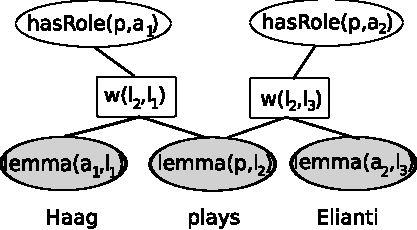
\includegraphics[scale=.70]{LocalFormula2}
\end{center}
\caption{Factor graph for the local formula in section \ref{sec:local}. Here round nodes represent variables (corresponding to the states of ground atoms) and the rectangular nodes represent ground formulae and their weights.}
\label{fig:local2}
\end{figure}

\subsection{Global formulae}
\label{sec:global}

\emph{Global} formulae relate several hidden ground atoms. We use this type of formula for two purposes: to ensure consistency between the predicates of all SRL stages, and to capture some of our background knowledge about SRL. We will refer to formulae that serve the first purpose as \emph{structural constraints}. 

For example, a structural constraint is given by the (deterministic) formula
\[role(p,a,r) \Rightarrow hasRole(p,a)\]
which ensures that, whenever the argument $a$ is given a label $r$ with respect to the predicate $p$, this argument must be an argument of $a$ as denoted by \emph{hasRole(p,a)}. Note that this formula by itself models the traditional ``bottom-up'' argument identification and classification pipeline: it is possible to not assign a role $r$ to an predicate-argument pair $(p,a)$ proposed by the identification stage; however, it is impossible to assign a role $r$ to token pairs $(p,a)$ that have not been proposed as potential arguments.

An example of another class of structural constraints is 
\[
hasRole(p,a)\Rightarrow\exists r.role(p,a,r)
\]
which, by itself, models an inverted or ``top-down'' pipeline. In this architecture the argument classification stage can assign roles to tokens that have not been proposed by the argument identification stage. However, it must assign a label to any token pair the previous stage proposes. 
%IV
Figure \ref{fig:global2} illustrates the structural formulae we use in form of a Markov Network.

\begin{figure}[ht]
\begin{center}
   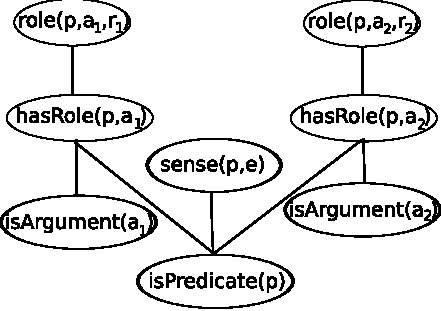
\includegraphics[scale=.70]{GlobalFormula2}
\end{center}
\caption{Markov Network that illustrates the structural constraints we use.}
\label{fig:global2}
\end{figure}

For the SRL predicates that perform a labelling task (\emph{role} and \emph{sense}) we also need a structural constraint which ensures that not more than one label is assigned. For instance,
\[
(role(p,a,r_1) \wedge r_1 \neq r_2 \Rightarrow \neg role(p,a,r_2)  )
\]
forbids two different semantic roles for a pair of words. 

There are three global formulae that capture our linguistic background knowledge. The first one is a deterministic constraint that be been frequently applied in the SRL literature. It forbids cases where distinct arguments of a predicate have the same role unless the role describes a modifier:
\begin{eqnarray*}
 &role\left(p,a_{1},r\right)\wedge \neg mod\left(r\right)\wedge a_{1}\neq a_{2}  \Rightarrow\\
  & \neg role\left(p,a_{2},r\right)
\end{eqnarray*}

The second ``linguistic'' global formulae is
\[
role(p,a,+r) \wedge lemma(p,+l) \Rightarrow sense(p,+s) 
\]
which implies that when a predicate $p$ with lemma $l$ has an argument $a$ with role $r$ it has to have the sense $s$. Here the weight depends on the combination of role $r$, lemma $l$ and sense $s$.

The third and final ``linguistic'' global formulae is
\begin{eqnarray*}
  & lemma(p,+l) \wedge ppos(a,+p)  \\
  & \wedge hasRole(p,a)  \Rightarrow sense(p,+f) 
\end{eqnarray*}
It implies that if a predicate $p$ has the lemma $l$ and an argument $a$ with POS tag $p$ it has to have the sense $s$. This time the weight depends on the combination of POS tag $p$, lemma $l$ and sense $s$.

Note that the final two formulae evaluate the semantic frame of a predicate and become local formulae in a pipeline system that performs sense disambiguation after argument identification and classification.

Table \ref{tbl:global} summarises the global formulae we use in this work. 

\begin{table*}[ht]
    \centering
    \small
    \begin{tabular}{|c|l|}\hline
        \multirow{4}{*}{Bottom-up}     
       & $sense(p,s) \Rightarrow predicate(p)$\\
       & $hasRole(p,a) \Rightarrow predicate(p)$\\
       & $hasRole(p,a) \Rightarrow argument(a)$\\
       & $role(p,a,r) \Rightarrow hasLabel(p,a)$\\\hline
       \multirow{4}{*}{Top-Down } &       $isPredicate(p) \Rightarrow\exists s.sense(p,s)$\\
       & $isPredicate(p) \Rightarrow\exists a.hasRole(p,a)$\\
       & $isArgument(a)  \Rightarrow\exists p.hasRole(p,a)$\\
       & $hasLabel(p,a) \Rightarrow\exists r. role(p,a,r)$\\\hline
       \multirow{2}{*}{Unique Labels }  
       
       & $role(p,a,r_1) \wedge r_1 \neq r_2 \Rightarrow \neg role(p,a,r_2)$\\
       & $sense(p,s_1) \wedge s_1 \neq s_2 \Rightarrow \neg sense(p,r_2) $\\\hline
         \multirow{3}{*}{Linguistic} 
       & $role\left(p,a_{1},r\right)\wedge \neg mod\left(r\right)\wedge a_{1}\neq a_{2}  \Rightarrow \neg role\left(p,a_{2},r\right) $ \\
       & $ lemma(p,+l) \wedge ppos(a,+p) \wedge hasRole(p,a)  \Rightarrow sense(p,+f) $ \\
       & $ lemma(p,+l) \wedge role(p,a,+r) \Rightarrow sense(p,+f) $ \\
        \hline
    \end{tabular}
    \caption{Global formulae for ML model}
    \label{tbl:global}
\end{table*}



%For the predicates \emph{isPredicate} and \emph{isArgument} we define the
%following formuale:
%\begin{description}
    %\item[$Word$] a rule for the orthography of possible predicate or argument.
    %\item[$Lemma_{-2,-1,1,2}$] for each lemma in a window of two previous and two following token a rule of possible predicate or argument.
    %\item[$POSs_{-2,-1,1,2}$] for each POS in a window of two previous and two following tokens a rule of possible predicate or argument.
    %\item[$CoarsePOS$] a rule for the previous and the following coarse POS tags of possible predicate or argument.
    %\item[$CoarsePOS_2$] a rule for the two previous and two following corar POS tags of possible predicate or argument.
    %\item[$DependecyChildren$] a rule for the dependencies of each child of possible predicate or argument.
    %\item[$DependecyParent$] a rule for the dependencies of parent of possible predicate or argument.
    %\item[$DependecyChildrenPOS$] a rule for the POS tag for each child  of possible predicate or argument.
    %\item[$DependecyChildrenParPOS$] a rule for the POS tag of parent and each child  of possible predicate or argument.
    %\item[$MFrame$] a rule for the MFrame of possible predicate or argument.
%\end{description}

%For the predicate \emph{hasRole} we define the following formulae:
%\begin{description}
    %\item[*$Lemma$] a rule for the lemmas of possible predicate and argument.
    %\item[*$POS$] a rule for the POS tags of possible predicate and argument.
    %\item[*$LemmaPOS$] a rule for the lemma of possible predicate and POS of possible argument.
    %\item[*$POSLemma$] a rule for the POS of possible predicate and lemma of possible argument.
    %\item[$SameLemma$] a rule if possible predicate and argument share the same
        %lemma.
    %\item[*$SamePOS$] a rule if possible predicate and argument share the same
        %POS.
    %\item[*$CorsePosTags$] a rule for each combination of coarse POS of pair of token after or before the possible predicate and argument.
    %\item[$POSArg_{-1,+1}$] for the previous and following POS tags of tokens of a possible argument
        %a rule with the POS tag of a possible predicate.
    %\item[$BinDistance_{0,1,2,3,4,5,10}$] a rule for the bin distances among possible predicate and argument.
    %\item[*$VoiceBinDistance_{0,1,2,3,4,5,10}$] a rule for the bin distances among possible predicate and argument and the voice of the possible predicate.
    %\item[$PalmePruned(POS)$] a rule if the possible predicate and argument are
        %pruned by palmer heuristic (extra version with POS tag for predicate).
    %\item[$Dependency$] for possible predicate and argument a rule for their
        %syntactic dependency.
    %\item[*$Dependencies(Voice)$] a rule for syntactic dependencies for both possible predicate and
        %argument (extra version with voice).
    %\item[$PathLength_{0,1,2,3,4,5,10}$] A rule for each bin of the length of the path among the possible predicate and possible
        %argument.
    %\item[*$DepPath(Voice)$] a rule for the dependency path among the
        %possible predicate and possible argument (extra version for voice).
    %\item[*$UnlabelledDepPath(Voice,Lemma)$] a rule for the unlabelled dependency path frame among the
        %possible predicate and possible argument (extra versions for voice and
        %lemma of predicate and argument).
    %\item[*$DepPathFrame(Voice,Lemma)$] a rule for the dependency path frame among the
        %possible predicate and possible argument (extra versions for voice and
        %lemma of predicate).
    %\item[*$PairUnlabelledDepPathFrame(Lemma)$] a rule for the unlabelled dependency path frame among the
        %possible predicate and possible argument (extra versions for lemma of
        %predicate and arguments).
    %\item[$SamePath$] a rule for the dependency path among the
        %possible predicate and possible argument if both are the same.
    %\item[$SamePathFrame$] a rule for the dependency path frame among the
        %possible predicate and possible argument if both are the same.
    %\item[*$PPattachment$] for the combination of lemma and POS the child of prepositional phrase as possible argument and possible predicate.
%\end{description}
%The formulae with the star symbol at the start was defined for the \emph{role}
%predicate as well. Additionally, for the role we define:
%\begin{description}
    %\item[$POS$] a rule for both POS tags of possible predicate and the bin
        %distance to the argument.
    %\item[$POSPOS$] a rule for the POSs of possible predicate and argument.
    %\item[*$Dependencies_{0,1,2,3,4,5,10}$] a rule for bin distances and the syntactic dependencies for both possible predicate and
        %argument (extra version with voice).
    %\item[$POSPOS_{0,1,2,3,4,5,10}$] a rule for the POS and the bin distances among  possible predicate and argument.
    %\item[$BinDistance(Lemmma,Voice)_{0,1,2,3,4,5,10}$] a rule for the bin distances among possible predicate and argument with their lemmas and/or voice.
    %\item[*$DepPath(Lemma,CorsePos)$] a rule for the dependency path among the
        %possible predicate and possible argument with lemma (extra version for coarse POS, and lemma argument).
    %\item[$DepPathDistance(Voice,Lemma)_{0,1,2,3,4,5,10}$] a rule for bin distance among the dependency path of the
        %possible predicate and possible argument (extra versions for voice and
        %lemma of predicate).
    %\item[$DepPathFrameDistance(Voice,Lemma)_{0,1,2,3,4,5,10}$] a rule for bin distance among the dependency path frame of the
        %possible predicate and possible argument (extra versions for voice and
        %lemma of predicate).
%\end{description}

%Finally, we define the following local formulae for the \emph{sense} predicate:
%\begin{description}
    %\item[$sense$] a rule for the sense of a possible predicate.
    %\item[$lemma$] a rule for the sense of a possible predicate and its lemma.
%\end{description}




% Finally, to our last group of rules belongs the soft formulae and hard constrains with extra linguistic knowledge. Figure \ref{fig:global2} shows an example of soft formulae. An example, of hard constriain which uses extra linguistic knowledge is:
% \begin{eqnarray*}
%  & role\left(p,a_{1},r\right)\wedge arg\left(r\right)\wedge a_{1}\neq a_{2} & \Rightarrow\\
%   & \neg role\left(p,a_{2},r\right)
% \end{eqnarray*}
% In this case we constrain to one semantic role to the words identify as proper arguments by the Palmer's heuristics. % ??
%
%We have slit our global formulae into four groups. The first, are hard constrains which only involve one hidden predicate. The second one correspond to the hard constrains which involve more than one hidden predicate but follow a bottom-up strategy. This is conect two hidden predicates following the pipeline of the stages of the task. The top-down group group goes in a different direction. And finally, the fourth group contains the global formulae. In the section \ref{sec:results} we will explore how these relations contribute to the whole model. Table \ref{tbl:global} enumerate the global formulae used in this work.
%\begin{table}
%\begin{tabular}{|l|p{6cm}|}\hline
%Group & Description \\\hline
%1st   & There is one or less $role$ predicates for a pair of words (see Figure \ref{fig:hard1}.)\\
%      & There is one or less $frameLabel$ predicates for a word\\
%      & There are more than one $haslabel$ predicate for each word which is a possible argument by the Palmer heuristics\\\hline
%2nd   & If there is a $isPredicate(p)$ predicate, there must be a $frameLabel(p,_)$ predicate\\
%      & If thrre is a $isPredicate(p)$ predicate, there must be a $hasLabel(p,_)$ predicate\\      
%      & If there is a $hasLabel(p,a,_)$ predicate, there must be a $role(p,a,_)$ predicate\\\hline
%3rd   & If there is a $role(p,a,_)$ predicate, there must be a $hasLabel(p,a)$ predicate. \\
%      & If there is a $frameLabel(p,_)$ predicate, there must be a $isPredicate(p)$ predicate\\
%      & If there is a $hasLabel(p,_)$ predicate, there must be a $isPredicate(p)$ predicate.\\
%      & If there is a $hasLabel(_,a)$ predicate, there must be a $isArgument(a)$ predicate.\\\hline
%4th   & There shouldn't be two $hasLabel$ predicate for the which have as a predicate the same word, and the two arguments are prepositional phrases.\\
%      & There shouldn't be two predicates which overlap\\
%      & A $frameLabel$ predicated depends of the POS tags of the arguments of the predicate (see Figure \ref{fig:global1}\\
%      & For each proper argument defined by the Palmer heuristics there should be at most one $role$ predicate for that argument\\\hline
%      \end{tabular}
%\caption{Global formulae }
%\label{tbl:global}
%\end{table}
%


